\errorcontextlines=9
\documentclass{beamer}

\usepackage[T1]{fontenc}
\usepackage[utf8]{inputenc}
\usepackage[italian]{babel}

\usepackage{fontawesome5}
\usepackage{blkarray} %

\usepackage{mathtools}
%\usepackage{commath}


\usepackage{wrapfig}

\usetheme{Padova}

\title{Ricerca testuale estesa su corpus di piccole dimensioni}
\subtitle{Dipartimento di Matematica "Tullio Levi-Civita" \\ Università degli Studi di Padova \\ Corso di Laurea in Informatica}
%\institute[Universita di Padova]{Dipartimento di Matematica}
\author{Laureando: Andrea Nalesso}
\date{18 Dicembre 2019}
%\author{\hspace{\fill}Andrea Nalesso\hspace*{\fill}}
%\date{\hspace{\fill}18 Dicembre 2019\hspace*{\fill}}

\patchcmd{\theorem}{Theorem}{Teorema}{}{}
\begin{document}

	\maketitle

%	\begin{frame}{Indice}
%		\tableofcontents
%	\end{frame}

	\section{Azienda}
	\begin{frame}
		\frametitle{Azienda}
	  \begin{columns}
		\begin{column}{0.5\textwidth}
		   Prima software house italiana
		   \begin{itemize}
			\item 800M di fatturato
			\item oltre 1000 Partner
			\item oltre 130.000 clienti
			\item 5500 addetti
			\item partner in 50 paesi nel mondo
		   \end{itemize}
		   \vspace*{1em}
		   \hspace*{1em}Sede di Padova
		   \begin{itemize}
			   \item R\&D
			   \item rapporto diretto con il CTO
		   \end{itemize}
		\end{column}
		\begin{column}{0.5\textwidth}  %%<--- here
			\vspace{-11	em}
			
			\begin{figure}
				\centering
				
\includegraphics[width=\textwidth]{img/logo_azienda.png}
				%\caption{Indice}
			\end{figure}
			 
		\end{column}
	  \end{columns}
	\end{frame}

	\section{Progetto}
	\begin{frame}
		\frametitle{Progetto}
		\begin{figure}
			\vspace{-2em}
			\centering
			
\includegraphics[width=0.65\textwidth]{img/ztube.png}
			%\caption{Indice}
		\end{figure}
		\vspace{-2em}
		\begin{columns}[T]
			\begin{column}{0.4\textwidth}
				\begin{itemize}
					\item Ricerca nel corpus (formazione su prodotti aziendali)
				\end{itemize}
			\end{column}
			\begin{column}{0.33\textwidth}
				\centering
				\begin{itemize}
					\item word2vec: dati insufficienti
				\end{itemize}
			\end{column}
			\begin{column}{0.50\textwidth}
				\centering
				\begin{itemize}
					\item provare altri modi per migliorare la ricerca 
				\end{itemize}
			\end{column}
		\end{columns}
	\end{frame}

	\begin{frame}[fragile]
		\frametitle{Corpus}
		\vspace*{-1em}
		\begin{exampleblock}{Frammento audio -- Esempio}
		\begin{verbatim}
			{
				id: 205, start: 1276.2, end: 1293.5,
				text:
				  "Apri barcode 39 per poter utilizzare lo scanner 
				  collegato direttamente a client Bisogna installare 
				  sul client il componente di Desa Minecraft che per 
				  noi chiamiamo zitta scanner.",
				filename: "AAF-DMS-40-U03.mp4.srt"
			  }
		\end{verbatim}
	\end{exampleblock}
	\begin{columns}[T]
		\begin{column}{0.29\textwidth}
			\begin{itemize}
				\item 610 frammenti 
			\end{itemize}
		\end{column}
		\begin{column}{0.29\textwidth}
			\begin{itemize}
				\item 4h videolezioni
			\end{itemize}
		\end{column}
		\begin{column}{0.5\textwidth}
			\begin{itemize}
				\item errori di somiglianza fonetica
			\end{itemize}
		\end{column}
	\end{columns}
	\end{frame}

	\begin{frame}
		\frametitle{Soluzione}
		\begin{figure}
			%\vspace{-2em}
			\centering
			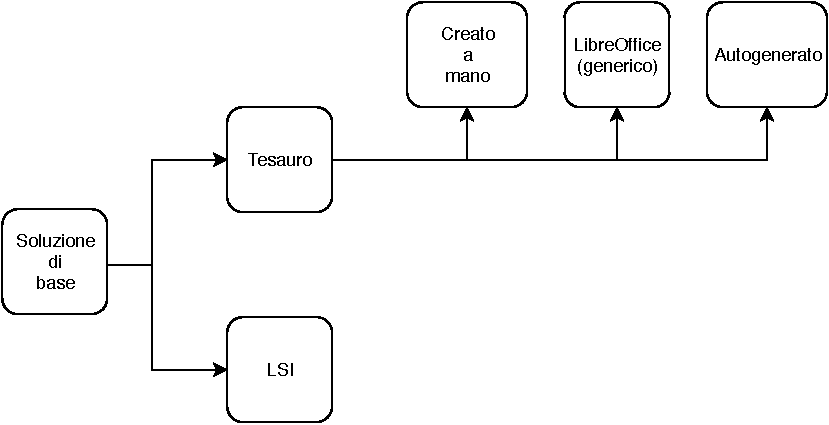
\includegraphics[width=\textwidth]{img/schema-soluzione.pdf}
			%\caption{Indice}
		\end{figure}
		\begin{itemize}
			\item Estrarre vs aggiungere contesto
		\end{itemize}	
	\end{frame}

	\section{Ricerca}
	\begin{frame}
		\frametitle{Ricerca}
		\begin{figure}
			%\vspace{-2em}
			\centering
			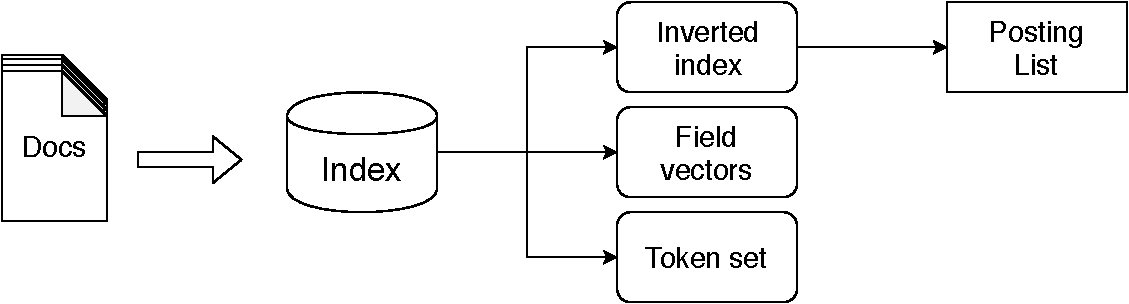
\includegraphics[width=\textwidth]{img/indice.pdf}
			%\caption{Indice}
		\end{figure}
		Indice	
		\begin{itemize}
			\item rappr. vettoriale di termini e documenti
				\item quali sono i token presenti
				\item in quali doc è presente un termine
			\end{itemize}
	\end{frame}

\section{Tesauro}
\begin{frame}
	\frametitle{Tesauro}

	%\begin{itemize}
		%\item Query Expansion: \texttt{token} \Rightarrow \texttt{[token]}
		\begin{description}
			\item[\textbf{Query Expansion}]: $\texttt{token} \Rightarrow \texttt{[token]}$	
		\end{description}
		\begin{block}{Score e normalizzazione}
		\vspace{-1em}
		\begin{columns}[T]
			\begin{column}{0.5\textwidth}
				\begin{equation*}
					\hspace*{1em}tf_{t,d} = 1 + log_2(|\{t \in T: t \in d\}|)
				\end{equation*}	
				\begin{equation*}
					\hspace{10em}tf\-idf_{t,d} = tf_{t,f} * idf_{t}
				\end{equation*}
			\end{column}
			\begin{column}{0.5\textwidth}
				\begin{equation*}
					\hspace*{-1em}idf_t = log_2(\frac{N}{|\{d \in D: t \in d\}|})
				\end{equation*}
			\end{column}
		\end{columns}
	\end{block}
	\vspace{1em}

	\begin{columns}[T]
		\begin{column}{0.5\textwidth}
			\textbf{Creato a mano}
			\begin{itemize}
				\item frequenze dei termini
				\item POS tagger
			\end{itemize}
		\end{column}
		\begin{column}{0.5\textwidth}
			\textbf{Generato}
			\begin{itemize}
				\item A: matrice termini documenti normalizzata
				\item C: matrice delle similarità
				\item $C = A * A^t$
			\end{itemize}
		\end{column}
	\end{columns}

%Query Expansion + due colonne (manuale, auto)
%	in auto metto pure tf-idf

\end{frame}

\section{LSI}
\begin{frame}
	\frametitle{LSI - parte 1}
	\begin{exampleblock}{2 concetti: internet e surf(sport)}
	\begin{columns}
		\begin{column}{0.7\textwidth}
			\begin{equation*}
				\textbf{A}=
				\begin{blockarray}{*{6}{c} l}
				  \begin{block}{*{6}{>{$\footnotesize}c<{$}} l}
					$D_1$ & $D_2$ & $D_3$ & $D_4$ & $D_5$ & $D_6$ & \\
				  \end{block}
				  \begin{block}{[*{6}{c}]>{$\footnotesize}l<{$}}
					1 & 1 & \textbf{\underline{0}} & 1 & 0 & 0 & internet \\
					1 & \textbf{\underline{0}} & 1 & 1 & 0 & 0 & web \\
					1 & 1 & 1 & 2 & 1 & 1 & surfing \\
					0 & 0 & 0 & 1 & 1 & 1 & beach \\
				  \end{block}
				\end{blockarray}
			  \end{equation*}
		\end{column}
		\begin{column}{0.3\textwidth}
			\begin{equation*}
				\textbf{B} = \begin{pmatrix}
					1 & 0 \\
					1 & 0 \\
					1 & 1 \\
					0 & 1 \\   
				\end{pmatrix}
			\end{equation*}
		\end{column}
	\end{columns}
\end{exampleblock}
$A$, $k$ tali che: 
\begin{itemize}
    \item  $A$: matrice termini-documenti $mxn$
    \item  $k <  rango(A)$
\end{itemize}

\begin{equation*}
		\textbf{A'} = argmin_{A'_{m x n} \text{con rango k}}  \lVert A - A' \rVert	
\end{equation*}
$ $

\end{frame}

\begin{frame}
	\frametitle{LSI - parte 2}
	\begin{theorem}[Esistenza della SVD]
		Data una matrice A qualsiasi di dimensione $m x n$ e rango $k$, esistono $U$, $S$, $V$ tali che $A = U \cdot S \cdot V$ , dove:
		\begin{itemize}
			\item $U$ è una matrice $m \cdot k$ con $U^T \cdot U = I_k$
			\item $S$ è una matrice diagonale $k \cdot k$
			\item $V$ è una matrice $k \cdot k$ con $V \cdot V^T = I_k$
		\end{itemize}
		\end{theorem}
		\begin{figure}
			%\vspace{-1em}
			\centering
			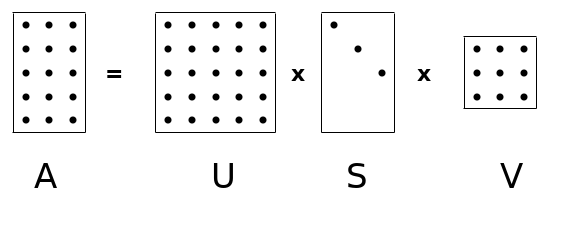
\includegraphics[width=0.8\textwidth]{img/SVD.png}
			%\caption{Indice}
		\end{figure}
\end{frame}

\section{Implementazione}
\begin{frame}
	\frametitle{Implementazione}
	\begin{figure}
		%\vspace{-2em}
		\centering
		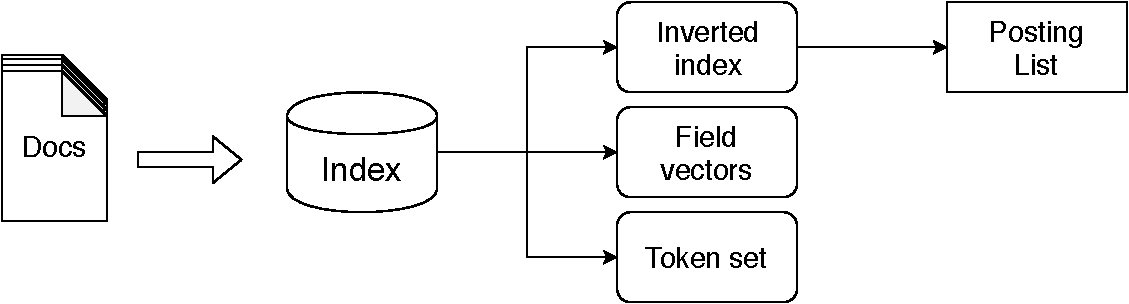
\includegraphics[width=\textwidth]{img/indice.pdf}
		%\caption{Indice}
	\end{figure}	
	\begin{itemize}
		\item Tesauro: Query Expansion ($\texttt{token} \Rightarrow \texttt{[token]}$)
		\item LSI: modifica \emph{field vectors}, \emph{inverted index}
	\end{itemize}

	\textbf{LALOLib} per SVD e calcoli matriciali
	
	\end{frame}

	\section{Librerie}
\begin{frame}
	\frametitle{Librerie}
	\begin{columns}
		\begin{column}{0.5\textwidth}
			
		\end{column}
	\end{columns}
	\begin{columns}
		\begin{column}{0.33\textwidth}
			\begin{figure}
				\vspace{-1em}
				\centering
				
\includegraphics[width=0.8\textwidth]{img/lunrjs.png}
				%\caption{Indice}
			\end{figure}
			\begin{figure}
				%\vspace{-2em}
				\centering
				
\includegraphics[width=0.8\textwidth]{img/numpy.png}
				%\caption{Indice}
			\end{figure}
			\begin{figure}
				%\vspace{-2em}
				\centering
				
\includegraphics[width=0.8\textwidth]{img/OpenNLP_Logo.pdf}
				%\caption{Indice}
			\end{figure}
		\end{column}
			\begin{column}{0.33\textwidth}
			\begin{figure}
				\vspace{-7em}
				\centering
				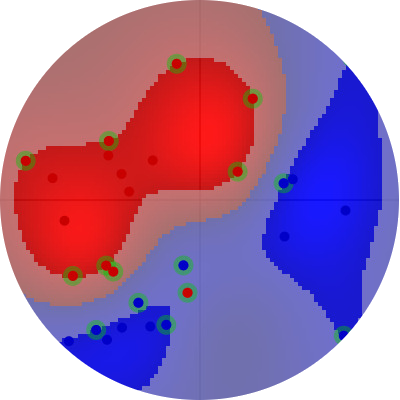
\includegraphics[width=0.8\textwidth]{img/lalolib.png}
				%\caption{Indice}
			\end{figure}
			\begin{figure}
				\vspace{-2em}
				\centering
				
\includegraphics[width=0.8\textwidth]{img/scikit-learn.png}
				%\caption{Indice}
			\end{figure}
			
		\end{column}
			\begin{column}{0.33\textwidth}
			\begin{figure}
				\vspace{-10em}
				\centering
				
\includegraphics[width=0.8\textwidth]{img/nodejs}
				%\caption{Indice}
			\end{figure}
		\end{column}
	\end{columns}

	

\end{frame}

\section{Prodotto finale}
\begin{frame}
	\frametitle{Prodotto finale}

	\begin{columns}
		\begin{column}{0.6\textwidth}
			\begin{figure}
				\vspace{-8em}
				\hspace*{1em}
				\centering
				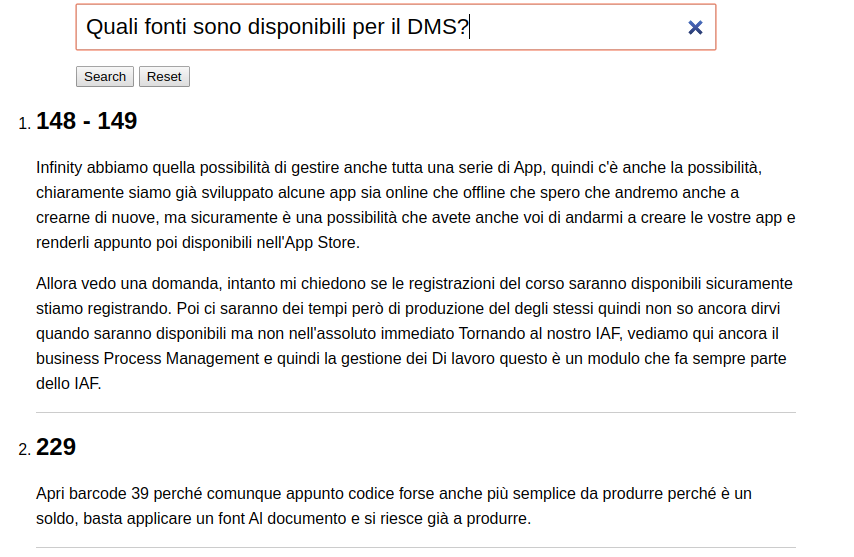
\includegraphics[width=\textwidth]{img/ricerca.png}
				%\caption{Indice}
			\end{figure}
		\end{column}
		\begin{column}{0.6\textwidth}
			\begin{figure}
				\vspace*{3em}
				\hspace{-2.5em}
				\centering
				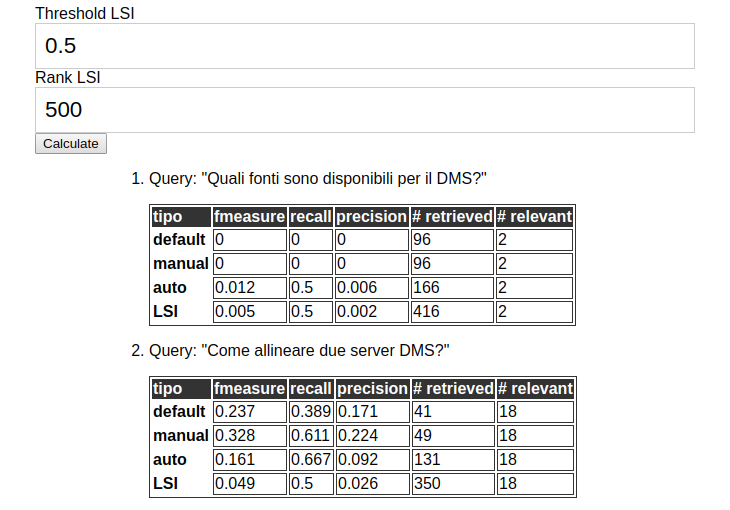
\includegraphics[width=\textwidth]{img/ir_eval.png}
				%\caption{Indice}
			\end{figure}
		\end{column}
	\end{columns}



\end{frame}

\section{Considerazioni finali}
\begin{frame}
	\frametitle{Considerazioni finali}


	\begin{columns}[T]
		\begin{column}{0.5\textwidth}
			Aspetti positivi:
			\begin{itemize}
				\item colmato lacune JS e acquisito basi di Node.js
				\item basi di recupero dell'informazione
				\item utilizzo libreria calcolo scientifico (LALOLib)
				\item autonomia nello studio e individuazione materiale
				\item ambiente collaborativo 
			\end{itemize}
		\end{column}
		
		\begin{column}{0.5\textwidth}
			Aspetti negativi:
	\begin{itemize}
		\item no implementazione autoencoder e ensamble
		\item soluzione naive è quella che paga di più
	\end{itemize}	
		\end{column}
	\end{columns}
\end{frame}

\begin{frame}
	\frametitle{Possibili estensioni}
	\begin{itemize}
		\item Considerare come documenti gruppi di frammenti audio
		\item Espandere il contesto usando Wikipedia
	\end{itemize}
	

\end{frame}

%	- inquadramento generale: azienda
%	- progetto nel quale il lavoro si inserisce
%	- problema specifico affrontato
%	- soluzione proposta
%	- implementazione (architettura, scelte progettuali) 
	

%	- strumenti utilizzati 
%	- considerazioni finali



%	\section{Introduction}
%
%	\begin{frame}{Introduction}
%
%		Etiam eu interdum ligula
%
%		Nunc mi eros, vulputate in ornare a, viverra eget quam \vspace{.5em}
%
%		\begin{itemize}
%			\item Morbi \textbf{vitae lacus} porta neque tincidunt sodales \vspace{.5em}
%			\item Proin tincidunt, \textbf{neque} at tincidunt mollis \vspace{.5em}
%			\item Ut \alert{lacinia sem a nibh} consequat porttitor
%		\end{itemize}
%	\end{frame}
%
%
%	\section{First section}
%
%	\begin{frame}{First section}
%		\begin{block}{Normal block}
%			Fusce luctus venenatis felis quis semper
%		\end{block}
%
%		\begin{alertblock}{Alert block}
%			$$ E = (x_1 \vee \neg x_2 \vee \neg x_3) \wedge (x_1 \vee x_2 \vee x_4) $$
%		\end{alertblock}
%
%		\begin{exampleblock}{Example block}
%			Proin tincidunt, neque at tincidunt mollis
%		\end{exampleblock}
%	\end{frame}


\end{document}
